\documentclass{beamer}

\usepackage[brazil]{babel}
\usepackage[utf8]{inputenc}
\usepackage[T1]{fontenc}
\usepackage{listings}

\usetheme{Madrid}
\setbeamertemplate{navigation symbols}{}

\lstset{
language=Python,
basicstyle=\ttfamily\tiny,
backgroundcolor=\color{white},
keywordstyle=\color{blue}\bfseries,
stringstyle=\color{red},
commentstyle=\color{green},
showspaces=false,
showstringspaces=false,
morekeywords={None,self,__init__},
literate=
{á}{{\'a}}1
{Á}{{\'A}}1
{à}{{\`a}}1 
{À}{{\`A}}1
{â}{{\^a}}1 
{Â}{{\^A}}1
{ã}{{\~a}}1
{Ã}{{\~A}}1
{ä}{{\"a}}1
{Ä}{{\"A}}1
{é}{{\'e}}1
{É}{{\'E}}1
{è}{{\`e}}1
{È}{{\`E}}1
{ê}{{\^e}}1
{Ê}{{\^E}}1
{ẽ}{{\~e}}1
{Ẽ}{{\~E}}1 
{ë}{{\"e}}1
{Ë}{{\"E}}1
{í}{{\'i}}1
{Í}{{\'I}}1
{ì}{{\`i}}1
{Ì}{{\`I}}1
{î}{{\^i}}1
{Î}{{\^I}}1
{ĩ}{{\~i}}1
{Ĩ}{{\~I}}1
{ï}{{\"i}}1
{Ï}{{\"I}}1
{ó}{{\'o}}1
{Ó}{{\'O}}1
{ò}{{\`o}}1
{Ò}{{\`O}}1
{ô}{{\^o}}1
{Ô}{{\^O}}1
{õ}{{\~o}}1
{Õ}{{\~O}}1
{ö}{{\"o}}1
{Ö}{{\"O}}1
{ú}{{\'u}}1
{Ú}{{\'U}}1
{ù}{{\`u}}1
{Ù}{{\`U}}1
{û}{{\^u}}1
{Û}{{\^U}}1
{ũ}{{\~u}}1
{Ũ}{{\~U}}1
{ü}{{\"u}}1
{Ü}{{\"U}}1
{ç}{{\c{c}}}1
{Ç}{{\c{C}}}1
}

\title[Estrutura de Dados]{Estrutura de Dados}

\author[Diego S. C. Nascimento]{Diego Silveira Costa Nascimento}

\institute[IFRN]{
Instituto Federal de Educação, Ciência e Tecnologia do Rio Grande do Norte\\
diego.nascimento@ifrn.edu.br
}

\date[\today]{\today}

\begin{document}

\begin{frame}[plain]
	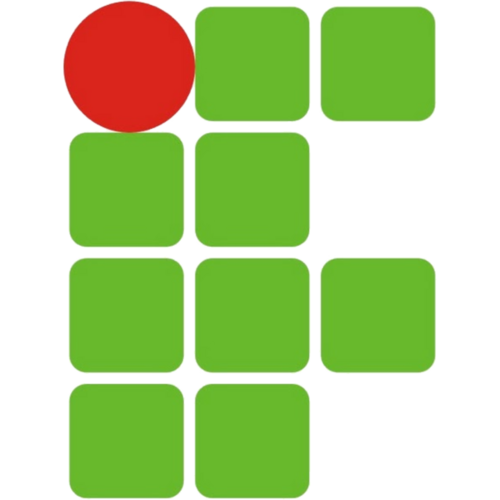
\includegraphics[scale=0.2]{IFRN}
	\titlepage
\end{frame}

\logo{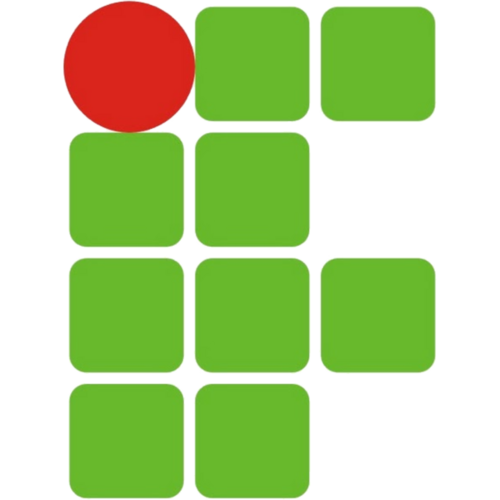
\includegraphics[scale=0.1]{IFRN}}

\begin{frame}
	\frametitle{Ementa do Curso}
  	\tableofcontents
\end{frame}

\AtBeginSection[]{
	\begin{frame}
		\frametitle{Ementa do Curso}
		\tableofcontents[currentsection]
	\end{frame}
}

\section{Introdução}

\begin{frame}
	\frametitle{Objetivos}
	
	\begin{itemize}
		\item Consolidar os conhecimentos sobre programação previamente
		adquiridos;
		\item Identificar e desenvolver modelos matemáticos, determinando que
		classes de problemas podem ser resolvidos com o uso deles;
		\item Criar representações concretas dos objetos e desenvolver rotinas
		capazes de atuar sobre essas representações, de acordo com o modelo
		considerado;
		\item Fornecer domínio de alocação dinâmica de memória;
		\item Apresentar as principais estruturas de dados: lista, fila, pilha, árvores e
		tabelas de dispersão;
		\item Introduzir aspectos básicos da complexidade de algoritmos;
		\item Apresentar os principais processos de ordenação e pesquisa de dados.
	\end{itemize}
\end{frame}

\begin{frame}
	\frametitle{Motivações}
	
	\begin{itemize}
		\item Proporciona reúso de código;
		\item Diminui custos de desenvolvimento e manutenção;
		\item Melhora o desempenho do sistema; e
		\item Organiza as informações.
	\end{itemize}
\end{frame}

\begin{frame}
\frametitle{Definições}

\begin{block}{Algoritmo}
É uma sequência finita e lógica de instruções ou passos, especificados em
uma determinada linguagem, que mostram como resolver determinado
problema.
\end{block}	\vfill

\begin{block}{Estrutura de Dados}
É um modo particular de armazenamento e organização de dados em um
computador de modo que possam ser usados de modo eficiente.
\end{block}	\vfill

\begin{block}{Programa}
É uma expressão em linguagem formal inteligível por um computador
(Algoritmos + Estruturas de dados).
\end{block}	
\end{frame}

\section{Ordenação}

\begin{frame}
\frametitle{Ordenação}

\begin{block}{Definição}
Uma ordenação consiste em colocar os elementos de um conjunto de dados
de forma organizada (ascendente ou descendente) de acordo seus valores.
\end{block}\vfill

\begin{itemize}
	\item Ordenação por inserção (Insert Sort);
	\item Ordenação por seleção (Select Sort);
	\item Ordenação por flutuação (Bubble Sort);
	\item Ordenação por mistura (Merge Sort); e
	\item Ordenação rápida (Quick Sort).
\end{itemize}

\end{frame}

\begin{frame}[fragile]
	\frametitle{Ordenação por Inserção}
	
	\begin{itemize}
		\item Eficiente quando aplicado a um pequeno número de elementos;
		\item Percorre um vetor de elementos da esquerda para a direita;
		\item À medida que avança vai deixando os elementos mais à esquerda
		ordenados; e
		\item Assemelha-se a ordenação de cartas de um jogo de baralho.
	\end{itemize}
	
	\begin{exampleblock}{Exemplo}
		\begin{lstlisting}
valores = [5, 8, 9, 2, 1]

for i in range(1,len(valores)):
    aux = valores[i]
    j = i
    while (j > 0) and (aux < valores[j -1]):
        valores[j] = valores[j - 1] 
        j -= 1
    valores[j] = aux

print(valores)
		\end{lstlisting}
	\end{exampleblock}
\end{frame}

\begin{frame}[fragile]
\frametitle{Ordenação por Seleção}

\begin{itemize}
	\item Baseado em passar sempre o menor valor do vetor para a primeira posição;
	\item Depois o de segundo menor valor para a segunda posição; e
	\item Assim é feito sucessivamente com os $(n - 1)$ elementos restantes.
\end{itemize}

\begin{exampleblock}{Exemplo}
	\begin{lstlisting}
valores = [5, 8, 9, 2, 1]

for i in range(0, len(valores) - 1):
    index_menor = i
    for j in range(i + 1, len(valores)):
        if valores[j] < valores[index_menor]:
            index_menor = j
    if valores[index_menor] < valores[i]:
        valores[i], valores[index_menor] = valores[index_menor], valores[i]  

print(valores)
	\end{lstlisting}
\end{exampleblock}
\end{frame}

\begin{frame}[fragile]
\frametitle{Ordenação por Flutuação}

\begin{itemize}
	\item A ideia é percorrer o vector diversas vezes;
	\item A cada passagem fazendo flutuar para o topo o maior elemento da
	sequência; e
	\item Essa movimentação lembra a forma como as bolhas em um tanque de
	água procuram seu próprio nível.
\end{itemize}

\begin{exampleblock}{Exemplo}
	\begin{lstlisting}
valores = [5, 8, 9, 2, 1]

for i in range(len(valores) - 1, 0, -1):
    for j in range(0, i):
        if (valores[j] > valores[j + 1]):
            valores[j], valores[j + 1] = valores[j + 1], valores[j] 

print(valores)
	\end{lstlisting}
\end{exampleblock}
\end{frame}

\begin{frame}
\frametitle{Ordenação por Mistura}

\begin{itemize}
	\item Do tipo dividir-para-conquistar;
	\item Dividir: Dividir os dados em subsequências pequenas; e
	\item Conquistar: Classificar as metades recursivamente aplicando o merge
	sort.
\end{itemize}
\end{frame}

\begin{frame}[fragile]
\frametitle{Ordenação por Mistura}

\begin{exampleblock}{Exemplo}
	\begin{lstlisting}
def merge_sort(lista):
    if len(lista) > 1:
        centro = len(lista) // 2
        sublista_esquerda = lista[:centro]
        sublista_direita = lista[centro:]

        merge_sort(sublista_esquerda)
        merge_sort(sublista_direita)

        i = j = k = 0
        while i < len(sublista_esquerda) and j < len(sublista_direita):
            if sublista_esquerda[i] < sublista_direita[j]:
                lista[k] = sublista_esquerda[i]
                i += 1
            else:
                lista[k] = sublista_direita[j]
                j += 1
            k += 1
        while i < len(sublista_esquerda):
           lista[k] = sublista_esquerda[i]
           i += 1
           k += 1
        while j < len(sublista_direita):
            lista[k] = sublista_direita[j]
            j += 1
            k += 1
	\end{lstlisting}
\end{exampleblock}
\end{frame}

\begin{frame}[fragile]
\frametitle{Ordenação por Mistura}

\begin{exampleblock}{Exemplo}
	\begin{lstlisting}
valores = [5, 8, 9, 2, 1]
merge_sort(valores)
print(valores)
	\end{lstlisting}
\end{exampleblock}
\end{frame}

\begin{frame}
\frametitle{Ordenação Rápida}

\begin{itemize}
	\item Escolha um elemento da lista, denominado pivô;
	\item Rearranje a lista de forma que todos os elementos anteriores ao pivô
	sejam menores que ele;
	\item Ao fim do processo o pivô estará em sua posição final e haverá duas
	sublistas não ordenadas; e
	\item Recursivamente ordena as sublistas de elementos menor e a maior.
	sort.
\end{itemize}
\end{frame}

\begin{frame}[fragile]
\frametitle{Ordenação Rápida}

\begin{exampleblock}{Exemplo}
	\begin{lstlisting}
def quick_sort(lista, index_inicio=None, index_fim=None):
    if index_inicio == None and index_fim == None:
        index_inicio = 0
        index_fim = len(lista) - 1

    pivo = lista[(index_inicio + index_fim) // 2]
    i = index_inicio
    j = index_fim

    while i < j:
        while lista[i] < pivo:
            i += 1

        while lista[j] > pivo:
            j -= 1

        if i < j:    
            lista[i], lista[j] = lista[j], lista[i]
        i += 1
        j -= 1

    if j > index_inicio:
        quick_sort(lista, index_inicio, j)
    if i < index_fim:
        quick_sort(lista, j+1, index_fim)
	\end{lstlisting}
\end{exampleblock}
\end{frame}

\begin{frame}[fragile]
\frametitle{Ordenação Rápida}

\begin{exampleblock}{Exemplo}
	\begin{lstlisting}
valores = [7,1,3,9,8,4,2,7,4,2,3,5]
quick_sort(valores)
print(valores)
	\end{lstlisting}
\end{exampleblock}
\end{frame}

\end{document}